\section{Optimización y experimentación}
En la siguiente sección, se evaluará el rendimiento de la base de datos mediante la ejecución de tres consultas complejas. Este análisis se llevará a cabo en varios escenarios que incluyen diferentes volúmenes de datos, y se realizarán pruebas sin índices, únicamente con los índices por defecto y con los índices que consideremos más adecuados para garantizar la ejecución óptima de estas consultas. Finalmente, se procederá a analizar y comparar los resultados obtenidos.
\subsection{Consultas SQL para el experimento}
\subsubsection{Descripción del tipo de consultas seleccionadas}
\begin{itemize}
	\item{\textbf{Consulta 1}: La siguiente consulta obtiene el nombre, email y número de celular de los directores actuales, así como la dirección, coordenadas y fecha de construcción de las 20 sedes más antiguas construidas entre 1990 y 2010, excluyendo aquellas sedes donde el número total de profesores y alumnos exceda 400.}
	      \begin{itemize}
		      \item{\textbf{Justificación}: La institución educativa está en un proceso de planificación para realizar renovaciones y mantenimiento en sus sedes. Se ha decidido comenzar con las sedes construidas entre los años 1990 y 2010, ya que estas son las que han demostrado tener más necesidad de atención. Para minimizar las interrupciones en las actividades escolares, se ha establecido que solo se seleccionarán aquellas sedes donde la suma del número de profesores y alumnos no exceda 400. Además, se requiere la información de los directores de estas sedes para coordinar las visitas de evaluación y supervisión.}
	      \end{itemize}
	\item{\textbf{Consulta 2}: Se desea conocer el nombre completo, bonificación, código de cuenta interbancaria e email de los colaboradores identificados como activos actualmente a los que les corresponde el bono que ofrece la institución. Para calcular la bonificación debemos tomar en cuenta que las sedes que este año están cumpliendo un aniversario múltiplo de 10 (sin contar al 0) ofrecen un bono de 5\%, respecto al pago mensual (el sueldo mensual se obtiene cuadruplicando la multiplicación del pago por hora por las horas semanales), para los colaboradores que nacieron entre 1960 y 1980. De existir un colaborador que labore en más de una sede se debe evaluar la condición del aniversario para todas las sedes; si se cumple la condición en más de una, debemos multiplicar el bono por el número de sedes en las que se cumpla.}
	      \begin{itemize}
		      \item{\textbf{Justificación}: La institución educativa tiene una política que consiste en que cada 10 años desde la construcción de cada sede se ofrece un bono de 5\%, respecto al pago mensual, a los colaboradores activos de mayor edad, que trabajan en esa sede. El área de finanzas debe realizar el desembolso de este bono; por ello, se necesita conocer el nombre completo, monto respectivo, código de cuenta interbancaria para realizar la transferencia de este, y su email para emitir el comprobante de pago.}
	      \end{itemize}
	\item{\textbf{Consulta 3}: Se desea conocer el nombre, primer apellido, segundo apellido, sexo e email de los alumnos menores de 18 años cuyo apoderado sea un colaborador registrado como activo, que trabaja a tiempo completo (más de 48 horas semanales) y cuyo sueldo mensual sea menor a 2000 soles (el sueldo mensual se obtiene cuadruplicando la multiplicación del pago por hora por las horas semanales). Además deben haber transcurrido como mínimo 2 años desde la matrícula del alumno.}
	      \begin{itemize}
		      \item{\textbf{Justificacion}: La institución educativa implementará la iniciativa de ofrecer un descuento especial en el pago mensual a los alumnos menores de edad cuyo apoderado sea un colaborador activo de la institución que labore a tiempo completo y su sueldo mensual sea menor a 2000. El alumno debe haber estado matriculado por lo menos 2 años antes del actual.}
	      \end{itemize}
\end{itemize}
\subsubsection{Implementación de consultas en SQL}
\begin{itemize}
	\item{\textbf{Consulta 1}:
	      \lstinputlisting[language=SQL]{code-snippets/query-1/query_1.sql.}}
	\item{\textbf{Consulta 2}:
	      \lstinputlisting[language=SQL]{code-snippets/query-2/query_2.sql}}
	\item{\textbf{Consulta 3}:
	      \lstinputlisting[language=SQL]{code-snippets/query-3/query_3.sql}}
\end{itemize}
\subsection{Metodología del experimento}
\begin{sloppypar}
	Primero, creamos cuatro esquemas: ``mil\_datos'', ``diezmil\_datos'', ``cienmil\_datos'' y ``millon\_datos''. Cada uno de estos esquemas contiene la cantidad de datos que su nombre indica.
\end{sloppypar}
\lstinputlisting[language=SQL]{code-snippets/create_schemas.sql}

Luego, ejecutaremos cada consulta en cada uno de los esquemas, primero, sin índices, segundo, con los índices por defecto y, finalmente, con los índices por defecto más los índices que consideremos más adecuados para garantizar la ejecución óptima de estas consultas.\\

Sin embargo, antes de ejecutar las consultas sin índice y con el índice por defecto, es necesario ejecutar el comando \textbf{DROP INDEX IF EXISTS}. Esto asegura que cualquier índice personalizado creado previamente no interfiera con las consultas. De esta manera, garantizamos que las consultas se realicen correctamente y que los resultados reflejen el rendimiento de las consultas con y sin los índices predeterminados de la base de datos. \\

Por cada consulta realizada, se aplica un \textbf{VACUUM FULL} a todas las tablas involucradas para asegurar que estas se reestructuren completamente, recuperando espacio no utilizado y mejorando la eficiencia de la base de datos. \\

Finalmente, mediremos el tiempo de ejecución usando el comando \textbf{EXPLAIN ANALYZE} para probar el rendimiento y analizaremos los planes de ejercución de cada consulta en cada uno de los escenarios mencionados.
\subsection{Optimización de consultas}
\subsubsection{Planes de índices para la primera consulta}
\begin{itemize}
	\item{Ejecución sin índices}
	      \queryExecutionPlanGroup{code-snippets/query-1/query_1_unindexed.sql}{figures/query-1/query_1_unindexed_mil_datos.png}{figures/query-1/query_1_unindexed_diezmil_datos.png}{figures/query-1/query_1_unindexed_cienmil_datos.png}{figures/query-1/query_1_unindexed_millon_datos.png}{figures/query-1-csv/query_1_unindexed_mil_datos.png}{figures/query-1-csv/query_1_unindexed_diezmil_datos.png}{figures/query-1-csv/query_1_unindexed_cienmil_datos.png}{figures/query-1-csv/query_1_unindexed_millon_datos.png}
	\item{Ejercución con índices por defecto}
	      \queryExecutionPlanGroup{code-snippets/query-1/query_1_indexed_default.sql}{figures/query-1/query_1_indexed_default_mil_datos.png}{figures/query-1/query_1_indexed_default_diezmil_datos.png}{figures/query-1/query_1_indexed_default_cienmil_datos.png}{figures/query-1/query_1_indexed_default_millon_datos.png}{figures/query-1-csv/query_1_indexed_default_mil_datos.png}{figures/query-1-csv/query_1_indexed_default_diezmil_datos.png}{figures/query-1-csv/query_1_indexed_default_cienmil_datos.png}{figures/query-1-csv/query_1_indexed_default_millon_datos.png}
	\item{Ejecución con índices por defecto más índices personalizados}
	      \queryExecutionPlanGroup{code-snippets/query-1/query_1_indexed_custom.sql}{figures/query-1/query_1_indexed_custom_mil_datos.png}{figures/query-1/query_1_indexed_custom_diezmil_datos.png}{figures/query-1/query_1_indexed_custom_cienmil_datos.png}{figures/query-1/query_1_indexed_custom_millon_datos.png}{figures/query-1-csv/query_1_indexed_custom_mil_datos.png}{figures/query-1-csv/query_1_indexed_custom_diezmil_datos.png}{figures/query-1-csv/query_1_indexed_custom_cienmil_datos.png}{figures/query-1-csv/query_1_indexed_custom_millon_datos.png}
	\item{Descripción de las ejecuciones}
	      \begin{itemize}
		      \item {\textbf{Sin índices}: Los planes de consulta para las tablas de 1k y 1M son similares entre sí, con una operación extra de Gather en el millón de datos, mientras que los planes de 10k y 100k son similares pero difieren en comparación con los de 1k y 1M. Para 1k datos, se inicia con un Nested Loop Inner Join entre director y colaborador, seguido de otro Nested Loop Inner Join con persona y luego con sede. Las filas de sede se filtran usando un Seq Scan basado en sede.construccion\_fecha, y se ejecutan subconsultas ``SubQuery Scan'' para contar las filas de profesor\_sede y alumno, limitando el resultado a aquellos donde la suma no exceda de 400. Estos resultados se ordenan ``Sort'' por sede.construccion\_fecha y se limita la salida a 20 filas. Para 10k datos, se cambia el orden, comenzando con un Nested Loop Inner Join entre director y colaborador, seguido de un Seq Scan sobre sede y un Nested Loop Inner Join con persona, aplicando las mismas subconsultas y limitando los resultados de manera similar. En 100k datos, el plan es similar al de 10k, pero se utiliza Parallel Seq Scan para manejar el mayor volumen de datos eficientemente, manteniendo las subconsultas y la ordenación de resultados. En el millón de datos, se observan los mismos pasos que en 100k, pero con el uso adicional de Parallel Seq Scan y Gather después del join para consolidar los resultados de las operaciones paralelas. En todos los casos, los planes dependen de Nested Loop Inner Join y Seq Scan, pero se aprovechan de operaciones paralelas a medida que el tamaño de los datos aumenta.}
		      \item {\textbf{Con índices por defecto}: Los planes de consulta para las tablas de 1k, 10k, 100k y 1M datos muestran diferencias significativas en los algoritmos utilizados. Para 1k datos, el plan comienza con un Seq Scan en sede, filtrando por construccion\_fecha y limitando con subconsultas que cuentan las filas de profesor\_sede y alumno. Luego, se realiza un Nested Loop con director y colaborador, seguido de un Index Scan en persona, usando quicksort para ordenar. En 10k datos, el plan también inicia con Seq Scan en sede, pero las subconsultas se ejecutan más frecuentemente, con múltiples Nested Loop y Index Scan, manteniendo quicksort para la ordenación. Para 100k datos, se introduce un Materialize y top-N heapsort para ordenar, utilizando intensivamente Nested Loop y Seq Scan, aumentando el costo por el mayor volumen de datos. En 1M datos, se emplea Index Scan en sede.construccion\_fecha, mejorando la eficiencia. Se usan Nested Loop y Materialize para manejar los datos masivos, con top-N heapsort para ordenar y un uso efectivo de índices. Las subconsultas siguen siendo esenciales para los filtros en todos los casos.}
		      \item {\textbf{Con índices por defecto más índices personalizados}: Los planes de consulta para tablas de 1k, 10k, 100k y 1M datos muestran optimizaciones significativas. Para 1k datos, el plan comienza con un Index Scan en sede utilizando el nuevo índice, seguido de un Seq Scan en profesor\_sede y alumno para las subconsultas de conteo, realizando después un Nested Loop con director y colaborador, y finalizando con un Index Scan en persona. Para 10k datos, el plan también usa Index Scan en sede, pero las subconsultas se ejecutan más veces, resultando en múltiples Nested Loop y Index Scan, mejorando la eficiencia comparada con la versión sin índice. En 100k datos, se utiliza Index Scan en sede, y el Materialize se introduce para manejar mejor los datos, con top-N heapsort para la ordenación. Finalmente, para 1M datos, se observa un uso intensivo del Index Scan en sede, con múltiples Nested Loop, Materialize y Index Scan en otras tablas, optimizando el rendimiento significativamente. En todos los casos, las subconsultas y el uso del índice nuevo mejoran notablemente la eficiencia de la consulta.}
	      \end{itemize}
\end{itemize}
\subsubsection{Planes de índices para la segunda consulta}
\begin{itemize}
	\item{Ejecución sin índices}
	      \queryExecutionPlanGroup{code-snippets/query-2/query_2_unindexed.sql}{figures/query-2/query_2_unindexed_mil_datos.png}{figures/query-2/query_2_unindexed_diezmil_datos.png}{figures/query-2/query_2_unindexed_cienmil_datos.png}{figures/query-2/query_2_unindexed_millon_datos.png}{figures/query-2-csv/query_2_unindexed_mil_datos.png}{figures/query-2-csv/query_2_unindexed_diezmil_datos.png}{figures/query-2-csv/query_2_unindexed_cienmil_datos.png}{figures/query-2-csv/query_2_unindexed_millon_datos.png}
	\item{Ejercución con índices por defecto}
	      \queryExecutionPlanGroup{code-snippets/query-2/query_2_indexed_default.sql}{figures/query-2/query_2_indexed_default_mil_datos.png}{figures/query-2/query_2_indexed_default_diezmil_datos.png}{figures/query-2/query_2_indexed_default_cienmil_datos.png}{figures/query-2/query_2_indexed_default_millon_datos.png}{figures/query-2-csv/query_2_indexed_default_mil_datos.png}{figures/query-2-csv/query_2_indexed_default_diezmil_datos.png}{figures/query-2-csv/query_2_indexed_default_cienmil_datos.png}{figures/query-2-csv/query_2_indexed_default_millon_datos.png}
	\item{Ejecución con índices por defecto más índices personalizados}
	      \queryExecutionPlanGroup{code-snippets/query-2/query_2_indexed_custom.sql}{figures/query-2/query_2_indexed_custom_mil_datos.png}{figures/query-2/query_2_indexed_custom_diezmil_datos.png}{figures/query-2/query_2_indexed_custom_cienmil_datos.png}{figures/query-2/query_2_indexed_custom_millon_datos.png}{figures/query-2-csv/query_2_indexed_custom_mil_datos.png}{figures/query-2-csv/query_2_indexed_custom_diezmil_datos.png}{figures/query-2-csv/query_2_indexed_custom_cienmil_datos.png}{figures/query-2-csv/query_2_indexed_custom_millon_datos.png}
	\item{Descripción de las ejecuciones}
	      \begin{itemize}
		      \item {\textbf{Sin índices}: Los planes de consulta para las tablas de 1k, 10k, 100k y 1M datos muestran diferencias significativas en la ejecución. Para 1k datos, el plan utiliza un Nested Loop Left Join entre colaborador y profesor, con un Seq Scan en colaborador y subconsultas que filtran por sede. Se realiza una materialización y un Seq Scan en persona para aplicar el filtro de nacimiento\_fecha, y un Seq Scan en profesor. Para 10k datos, se repite el uso de Nested Loop Left Join y Seq Scan en colaborador, pero con más iteraciones y materializaciones, incrementando los costos de la consulta. En 100k datos, el plan sigue siendo similar, pero se observa un aumento significativo en la cantidad de subconsultas y materializaciones necesarias. Finalmente, para 1M datos, el plan utiliza Seq Scan en persona y colaborador con múltiples Nested Loop Left Join y subconsultas, resultando en una mayor complejidad en la ejecución. En todos los casos, los Seq Scan y Nested Loop predominan, y la ausencia de índices y el uso de materializaciones incrementan los costos y la complejidad con el aumento del tamaño de los datos.}
		      \item {\textbf{Con índices por defecto}: Los planes de consulta para las tablas de 1k, 10k, 100k y 1M datos muestran diferencias significativas en los algoritmos utilizados, aunque comparten algunas similitudes clave. En todos los casos, se utiliza un Nested Loop Left Join, Hash Join, Seq Scan en colaborador, SubQuery Scan para filtrar por sede, y un Index Only Scan en profesor. En 1k datos, el plan comienza con un Nested Loop Left Join seguido de un Hash Join entre colaborador y persona, aplicando un Seq Scan en colaborador y un SubQuery Scan para filtrar por sede, con un Index Only Scan en profesor y finalizando con un agregado. Para 10k datos, además de las similitudes mencionadas, se introduce un Bitmap Heap Scan en profesor\_sede, manejando más registros y ajustando las subconsultas de manera más frecuente. En 100k datos, se observa un incremento en los costos debido al mayor volumen de datos, manteniendo las operaciones básicas, pero con un uso intensivo de Bitmap Heap Scan en profesor\_sede y ajustes en las subconsultas. Para 1M datos, se siguen utilizando las mismas operaciones básicas, pero el manejo del volumen de datos masivo se optimiza con un uso más intensivo de Index Only Scan, SubQuery Scan en colaborador y sede, y Bitmap Heap Scan en profesor\_sede, incrementando los costos y manteniendo la eficiencia a través de técnicas consistentes y escalables.}
		      \item {\textbf{Con índices por defecto más índices personalizados}: Los planes de consulta para las tablas de 1k, 10k, 100k y 1M datos muestran diferencias significativas en los algoritmos utilizados, aunque comparten algunas similitudes clave. En todos los casos, se utiliza un Nested Loop Left Join, Hash Join, Seq Scan en colaborador, SubQuery Scan para sede, y un Index Only Scan en profesor. Para 1k datos, el plan comienza con un Nested Loop Left Join seguido de un Hash Join entre colaborador y persona, aplicando un Seq Scan en colaborador y un SubQuery Scan para sede, con un Index Only Scan en profesor y finalizando con un agregado. En 10k datos, se introduce un Bitmap Heap Scan en persona usando el nuevo índice, junto con un Bitmap Heap Scan en profesor\_sede. En 100k datos, se mantiene el uso intensivo de Bitmap Heap Scan en persona y profesor\_sede, con costos incrementados debido al mayor volumen de datos. Para 1M datos, el plan incluye un uso intensivo de Bitmap Heap Scan en persona y profesor\_sede, además de Memoize para optimizar el escaneo de sede, incrementando los costos y manteniendo la eficiencia a través de técnicas consistentes y escalables.}
	      \end{itemize}
\end{itemize}
\subsubsection{Planes de índices para la tercera consulta}
\begin{itemize}
	\item{Ejecución sin índices}
	      \queryExecutionPlanGroup{code-snippets/query-3/query_3_unindexed.sql}{figures/query-3/query_3_unindexed_mil_datos.png}{figures/query-3/query_3_unindexed_diezmil_datos.png}{figures/query-3/query_3_unindexed_cienmil_datos.png}{figures/query-3/query_3_unindexed_millon_datos.png}{figures/query-3-csv/query_3_unindexed_mil_datos.png}{figures/query-3-csv/query_3_unindexed_diezmil_datos.png}{figures/query-3-csv/query_3_unindexed_cienmil_datos.png}{figures/query-3-csv/query_3_unindexed_millon_datos.png}
	\item{Ejecución con índices por defecto}
	      \queryExecutionPlanGroup{code-snippets/query-3/query_3_indexed_default.sql}{figures/query-3/query_3_indexed_default_mil_datos.png}{figures/query-3/query_3_indexed_default_diezmil_datos.png}{figures/query-3/query_3_indexed_default_cienmil_datos.png}{figures/query-3/query_3_indexed_default_millon_datos.png}{figures/query-3-csv/query_3_indexed_default_mil_datos.png}{figures/query-3-csv/query_3_indexed_default_diezmil_datos.png}{figures/query-3-csv/query_3_indexed_default_cienmil_datos.png}{figures/query-3-csv/query_3_indexed_default_millon_datos.png}
	\item{Ejecución con índices por defecto más índices personalizados}
	      \queryExecutionPlanGroup{code-snippets/query-3/query_3_indexed_custom.sql}{figures/query-3/query_3_indexed_custom_mil_datos.png}{figures/query-3/query_3_indexed_custom_diezmil_datos.png}{figures/query-3/query_3_indexed_custom_cienmil_datos.png}{figures/query-3/query_3_indexed_custom_millon_datos.png}{figures/query-3-csv/query_3_indexed_custom_mil_datos.png}{figures/query-3-csv/query_3_indexed_custom_diezmil_datos.png}{figures/query-3-csv/query_3_indexed_custom_cienmil_datos.png}{figures/query-3-csv/query_3_indexed_custom_millon_datos.png}
	\item{Descripción de las ejecuciones}
	      \begin{itemize}
		      \item {\textbf{Sin índices}: Los planes de consulta para las tablas de 1k, 10k, 100k y 1M datos muestran diferencias significativas en los algoritmos utilizados, aunque comparten algunas similitudes clave. En todos los casos, se utiliza un Nested Loop Semi Join, Seq Scan en persona, y Materialize en varios niveles de subconsultas. Para 1k datos, el plan inicia con un Nested Loop Semi Join entre persona y alumno, seguido de un Seq Scan en persona, un Nested Loop Semi Join entre alumno y matricula, y un Seq Scan en alumno, aplicando filtros y materializando subconsultas para apoderado y colaborador. En 10k datos, se introduce un HashAggregate para agrupar alumno.dni y un Nested Loop Semi Join entre alumno y apoderado, con un Seq Scan en matricula aplicando el filtro de year. En 100k datos, se mantiene el uso de HashAggregate y Nested Loop Semi Join, con un aumento en los costos y filas removidas por los filtros. Para 1M datos, el plan incluye un Nested Loop Semi Join entre persona y alumno, un HashAggregate en matricula para agrupar por alumno\_dni, y un Nested Loop Semi Join entre alumno y apoderado, con materialización de subconsultas y un Seq Scan en colaborador para aplicar los filtros de esta\_activo, horas\_semanales\_trabajo, y sueldo\_hora, demostrando un incremento significativo en costos y uso de recursos.}
		      \item {\textbf{Con índices por defecto}: Los planes de consulta para las tablas de 1k, 10k, 100k y 1M datos muestran diferencias significativas en los algoritmos utilizados, aunque comparten algunas similitudes clave. En todos los casos, se utilizan Nested Loop, HashAggregate, y Hash Semi Join. Para 1k datos, el plan comienza con un Nested Loop entre persona y alumno, seguido de HashAggregate y Hash Semi Join entre alumno y matricula, con un Seq Scan en alumno, un Hash Join entre apoderado y colaborador, y un Index Scan en persona. En 10k datos, se mantiene el mismo enfoque, pero con un aumento en el número de filas y el uso de memoria. En 100k datos, los costos y el uso de recursos aumentan significativamente, pero el flujo de operaciones sigue siendo similar. Para 1M datos, se introduce la paralelización con Gather y Parallel Hash Semi Join, con Parallel Seq Scan en alumno y matricula, y Parallel Hash Join entre apoderado y colaborador, además de un Index Scan en persona, demostrando un incremento significativo en costos y eficiencia en el manejo de grandes volúmenes de datos.}
		      \item {\textbf{Con índices por defecto más índices personalizados}: Los planes de consulta para las tablas de 1k, 10k, 100k y 1M datos muestran diferencias significativas en los algoritmos utilizados, aunque comparten algunas similitudes clave como el uso de Nested Loop, HashAggregate, y Hash Semi Join en todos los planes. Para 1k datos, el plan comienza con un Nested Loop entre persona y alumno, seguido de HashAggregate y Hash Semi Join entre alumno y matricula, con un Seq Scan en alumno, un Hash Join entre apoderado y colaborador, y un Index Scan en persona. En 10k datos, se mantiene el mismo enfoque, pero con la adición de Bitmap Heap Scan en colaborador utilizando el nuevo índice. En 100k datos, los costos y el uso de recursos aumentan significativamente, con el uso intensivo de Bitmap Heap Scan en colaborador. Para 1M datos, se introduce la paralelización con Gather y Parallel Hash Semi Join, con Parallel Seq Scan en alumno y matricula, y Parallel Hash Join entre apoderado y colaborador, además de un Parallel Bitmap Heap Scan en colaborador, demostrando un incremento significativo en costos y eficiencia en el manejo de grandes volúmenes de datos. En todos los casos, se realiza un Index Scan en persona usando el índice primario para buscar los resultados finales.}
	      \end{itemize}
\end{itemize}
\subsection{Plataforma de pruebas}
\begin{table}[H]
    \centering
    \begin{tabular}{|>{\raggedright\arraybackslash}m{4cm}|>{\raggedright\arraybackslash}m{6cm}|}
        \hline
        \textbf{Sistema Operativo} & Windows 11 64-bits  \\ \hline
        \textbf{RAM}               & 16 GB               \\ \hline
        \textbf{CPU}               & Intel Core i5-1235U \\ \hline
        \textbf{Capacidad SSD}     & 512 GB              \\ \hline
        \textbf{PostgreSQL}        & 16.2                \\ \hline
        \textbf{DataGrip}          & 2024.1.3            \\ \hline
        \textbf{Docker}            & 4.31.1              \\ \hline
    \end{tabular}
    \caption{Especificaciones plataforma de pruebas}
\end{table}

% TODO: Centrar esto xd
\subsection{Medición de tiempos}
\subsubsection{Sin índices}
\executionTimeTable{
    1 & 175.210 & 205.306 & 1459.966 & 114534.298 \\
    \hline
    2 & 169.214 & 216.402 & 1516.431 & 117201.023 \\
    \hline
    3 & 177.710 & 274.884 & 1432.166 & 112984.575 \\
    \hline
    4 & 164.512 & 227.705 & 1627.135 & 118647.252 \\
    \hline
    5 & 192.028 & 250.850 & 1530.447 & 110794.072 \\
    \hline
    Promedio & 175.7348 & 235.0294 & 1513.229 & 114832.24399 \\
    \hline
    Desviación estándar & 9.3607 & 27.94095 & 75.31508 & 75.31508


}{Consulta 1}

\executionTimeTable{
    1 & 345.052 & 652.664 & 44891.185 &  \\
    \hline
    2 & 302.450 & 677.999 & 45805.199 &  \\
    \hline
    3 & 45805.199 & 734.057 & 52669.867 &  \\
    \hline
    4 & 378.817 & 692.784 & 47687.895 &  \\
    \hline
    5 & 309.166 & 710.037 & 47245.607 &  \\
    \hline
    Promedio & 332.4116 & 693.5082 & 47659.9506 &  \\
    \hline
    Desviación estándar & 30.76274 & 30.93022 & 3015.70432 &


}{Consulta 2}

\executionTimeTable{
    1 & 167.540  & 315.738  & 912.975 & 58503.063 & 3931597.627 \\
    \hline
    2 & 175.244  & 343.664 & 988.522 & 57298.393 & 3701023.021 \\
    \hline
    3 & 204.936 & 279.833 & 846.328 & 56484.832 & 3880975.729 \\
    \hline
    4 & 185.714 & 321.168 & 883.048 & 56993.090 & 3619787.067 \\
    \hline
    5 & 206.292 & 303.995 & 909.574 & 57136.121 & 3881074.322 \\
    \hline
    Promedio & 187.9452 & 312.8796 & 908.08940 & 57283.0998 & 3802891.5532 \\
    \hline
    Desviación estándar & 17.37788 & 23.42840 & 57.43193 & 746.90762 & 134795.57485


}{Consulta 3}


\subsubsection{Con índices por defecto}
\executionTimeTable{
    1 & 0.251 & 6.257 & 396.624 & 23115.031 \\
    \hline
    2 & 0.197 & 5.320 & 335.431 & 24299.944 \\
    \hline
    3 & 0.233 & 5.137 & 349.104 & 25556.929 \\
    \hline
    4 & 0.172 & 5.994 & 341.882 & 25814.039 \\
    \hline
    5 & 0.217 & 5.048 & 379.886 & 25312.110 \\
    \hline
    Promedio & 0.214 & 5.5512 & 360.5854 & 24819.6106 \\
    \hline
    Desviación estándar & 0.03078 & 0.54139 & 26.38975 & 1112.51145


}{Consulta 1}

\executionTimeTable{
    1 & 0.402 & 15.265 & 635.171 & 18865.481 \\
    \hline
    2 & 0.514 & 15.353 & 657.373 & 20918.379 \\
    \hline
    3 & 0.356 & 0.356 & 720.721 & 18851.776 \\
    \hline
    4 & 0.384 & 18.379 & 625.819 & 20451.714 \\
    \hline
    5 & 0.483 & 19.401 & 677.966 & 18945.817 \\
    \hline
    Promedio & 0.4278 & 17.214 & 663.41 & 19606.6334 \\
    \hline
    Desviación estándar & 0.06748 & 1.84471 & 37.89260 & 998.82839


}{Consulta 2}

\executionTimeTable{
    1 & 0.326 & 2.826 & 26.550 & 124.261 \\
    \hline
    2 & 0.461 & 3.347 & 20.467 & 119.881 \\
    \hline
    3 & 0.361 & 2.632 & 25.670 & 112.850 \\
    \hline
    4 & 0.338 & 2.287 & 24.999 & 116.193 \\
    \hline
    5 & 0.351 & 2.979 & 24.037 & 125.580 \\
    \hline
    Promedio & 0.3674 & 2.8142 & 24.3446 & 119.753 \\
    \hline
    Desviación estándar & 0.05396 & 0.39443 & 2.35473 & 5.35297


}{Consulta 3}

\subsubsection{Con índices por defecto más índices personalizados}
\executionTimeTable{
    1 & 0.161 & 4.324 & 82.715 & 652.607 \\
    \hline
    2 & 0.167 & 4.869 & 88.989 & 632.291 \\
    \hline
    3 & 0.153 & 4.892 & 86.286 & 605.283 \\
    \hline
    4 & 0.150 & 4.993 & 70.504 & 636.185 \\
    \hline
    5 & 0.159 & 4.811 & 81.153 & 633.012 \\
    \hline
    Promedio & 0.158 & 0.158 & 81.9294 & 631.87560 \\
    \hline
    Desviación estándar & 0.00670 & 0.26206 & 7.08127 & 17.00729
}{Consulta 1}

\executionTimeTable{
    1 & 0.279 & 14.750 & 590.168 & 16914.586 \\
    \hline
    2 & 0.263 & 16.133 & 610.265 & 16854.632 \\
    \hline
    3 & 0.241 & 14.500 & 581.118 & 17035.101 \\
    \hline
    4 & 0.306 & 13.077 & 570.728 & 16685.816 \\
    \hline
    5 & 0.224 & 14.478 & 563.422 & 16854.632 \\
    \hline
    Promedio & 0.2626 & 14.5876 & 583.1402 & 16868.95340 \\
    \hline
    Desviación estándar & 0.03205 & 1.08584 & 18.24900 & 126.13174
}{Consulta 2}

\executionTimeTable{
    1 & 0.269 & 1.716 & 23.353 & 93.977 \\
    \hline
    2 & 0.252 & 1.646 & 22.853 & 98.822 \\
    \hline
    3 & 0.239 & 1.849 & 17.552 & 104.173 \\
    \hline
    4 & 0.385 & 1.919 & 17.063 & 95.269 \\
    \hline
    5 & 0.262 & 1.812 & 18.207 & 105.109 \\
    \hline
    Promedio & 0.2814 & 1.7884 & 19.8056 & 99.47 \\
    \hline
    Desviación estándar & 0.05900 & 0.10817 & 3.04248 & 5.05365
}{Consulta 3}
\subsection{Resultados, análisis y discusión}
Debido a la gran escala de los datos, se ha dividdo los gráficos en dos partes para facilitar la visualización. Primero mostramos las que incluyen las estadísticas de las consultas sin índices, con índices por defecto y con índices por defecto más índices personalizados. Luego, realizamos la comparación entre estAs últimos dos.

Esta división se realizó porque, debido a la escala de las gráficas, la diferencia entre las consultas con índices por defecto y las consultas con índices personalizados no se evidencias en la primera imagen. Sin embargo, dicha diferencia sí existe y es importante resaltarla para un análisis más preciso.
\subsubsection{Consulta 1}
\begin{center}
	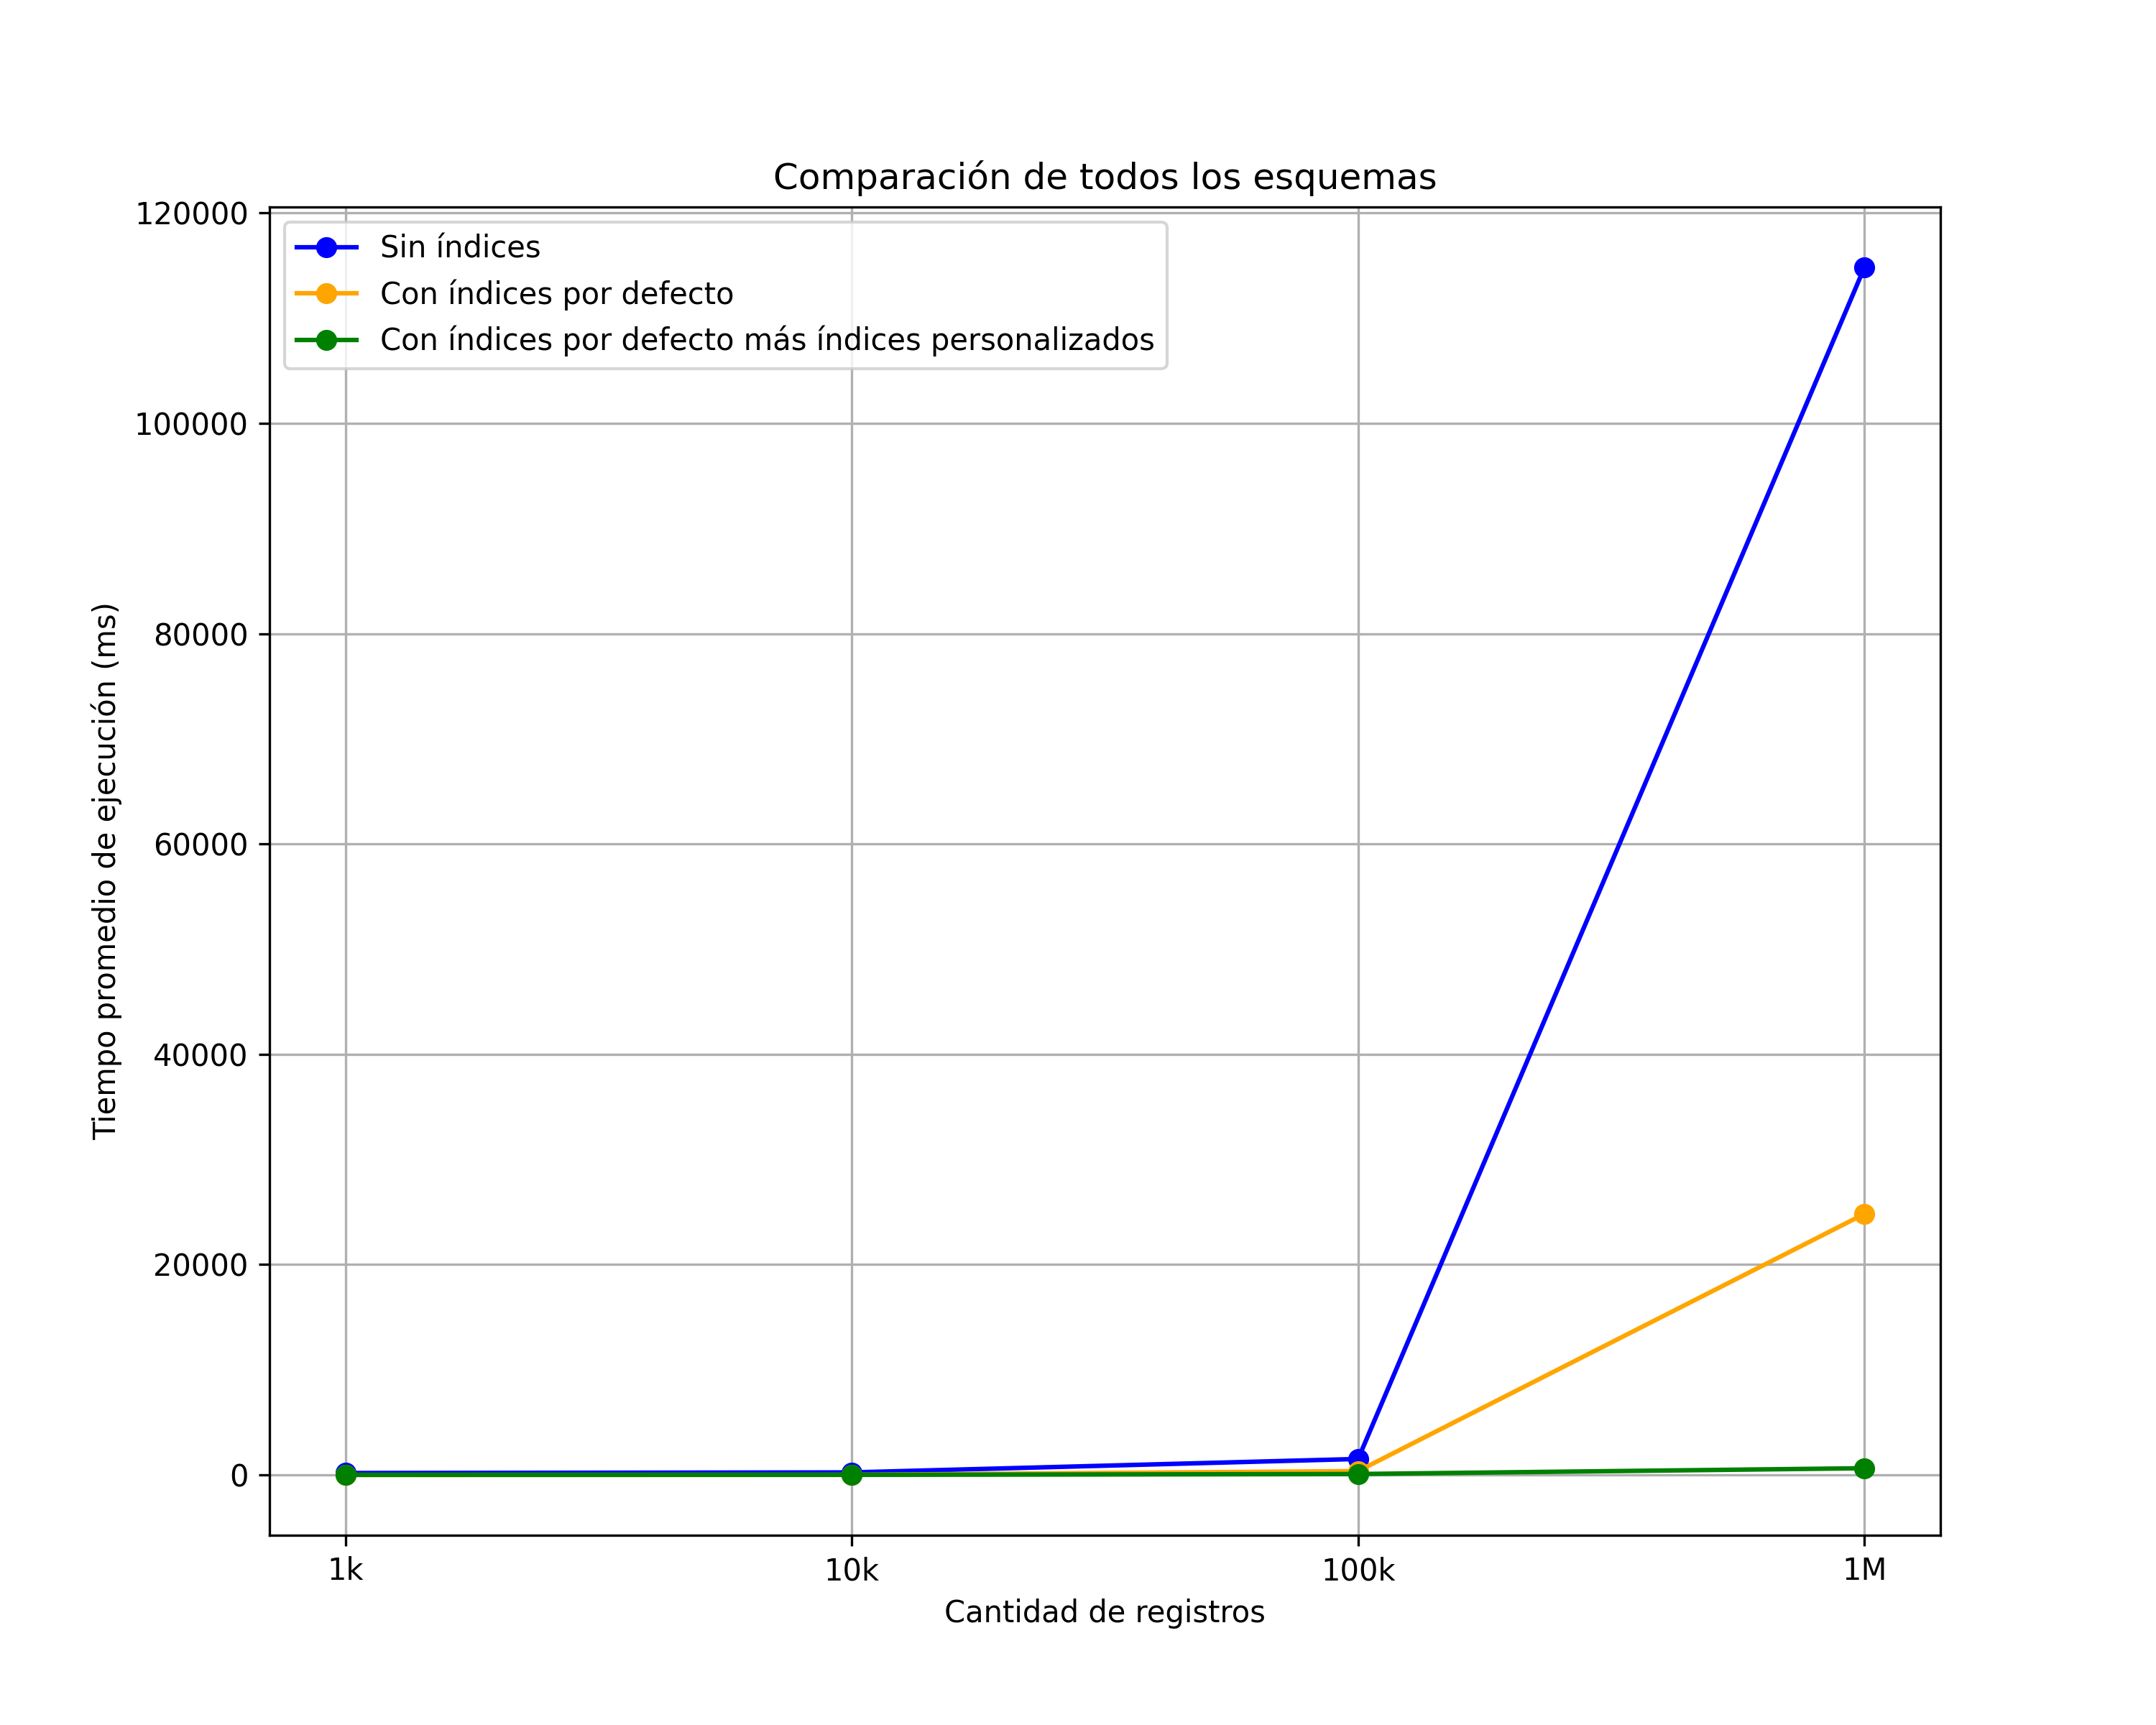
\includegraphics[width=\linewidth, keepaspectratio]{figures/query_1_execution_times_1.png}
	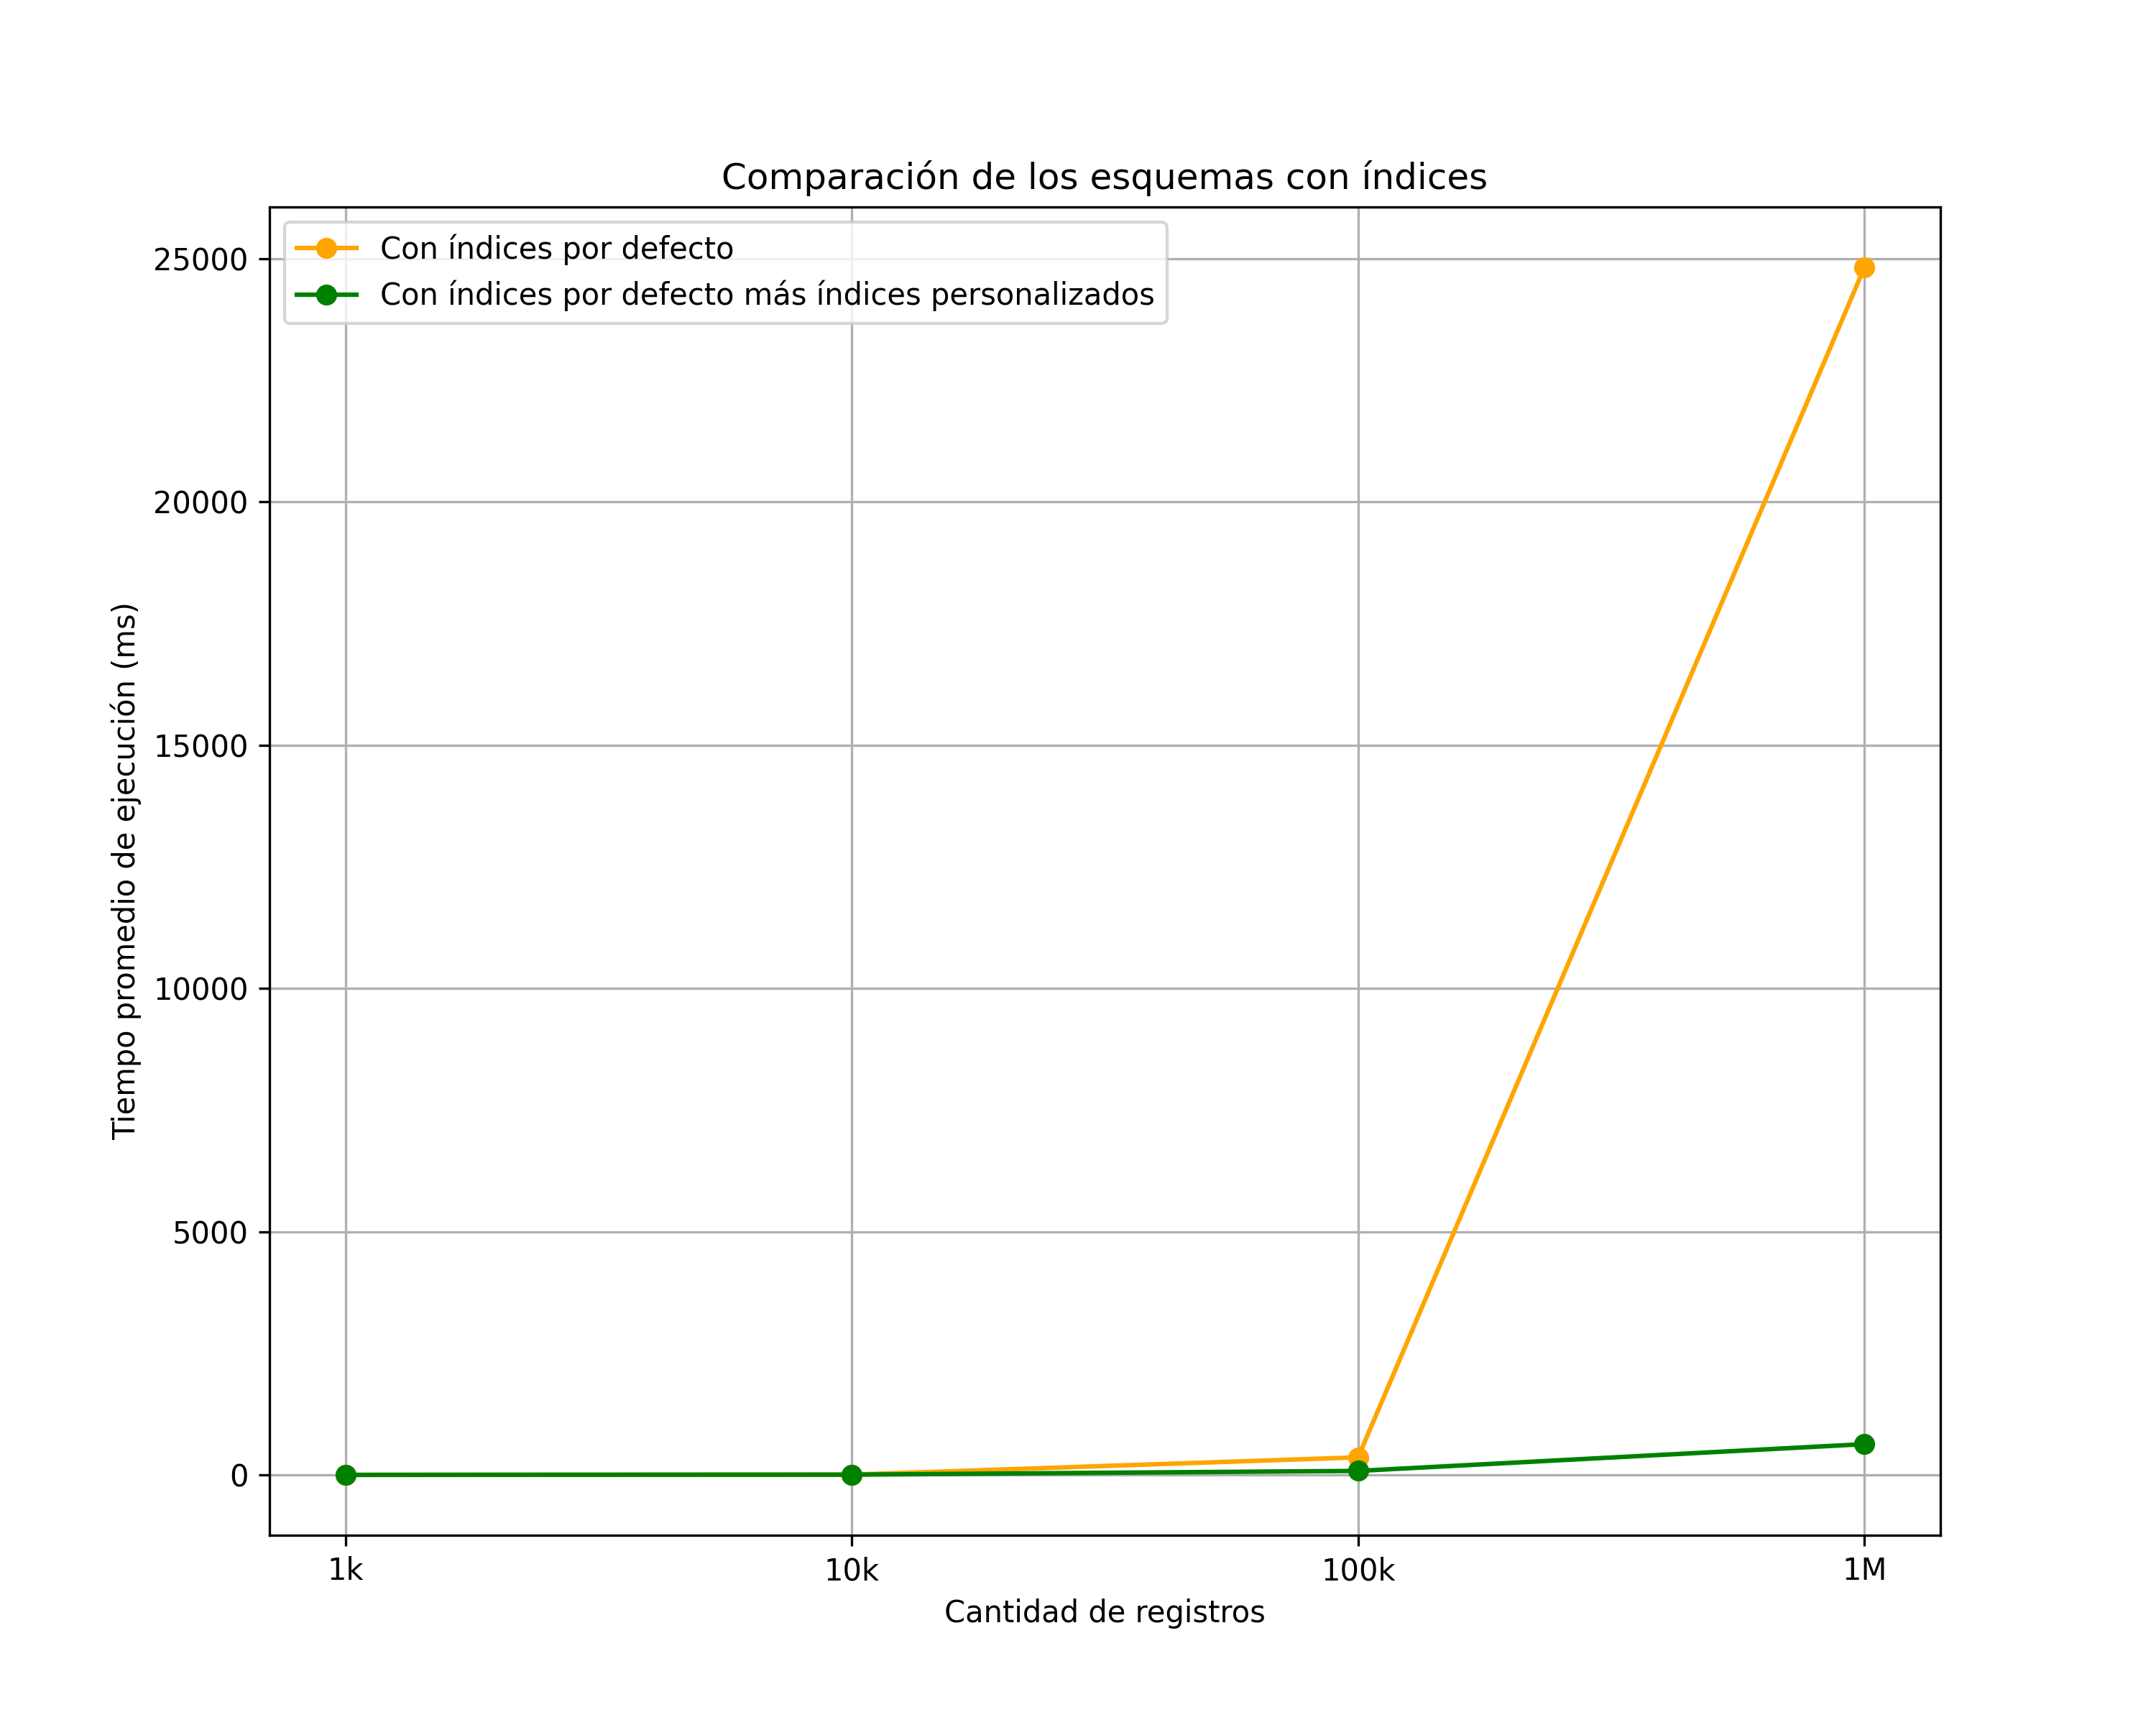
\includegraphics[width=\linewidth, keepaspectratio]{figures/query_1_execution_times_2.png}
\end{center}
Podemos observar una mejora significativa en los tiempos de ejecución entre las consultas sin índices y las consultas con índices (por defecto y por defecto más personalizado). Esto se debe a que en las consultas sin índices, estas dependen de escaneos secuenciales y uniones anidadas, incrementando exponencialmente el tiempo de ejecución por la gran cantidad de comparaciones necesarias. También identificamos una mejora entre las consultas con índices por defecto y las consultas con índices por defecto más índices personalizados: con índices por defecto, se utilizan escaneos de índice, reduciendo el tiempo de ejecución en un 78.38\% para un millón de datos, por otro lado, en el caso de los índices personalizados, la implementación de un índice en sede.construccion\_fecha permite una búsqueda más eficiente y reduce el número de filas examinadas, mejorando el tiempo de ejecución en un 97.45\% respecto a las consultas con índices por defecto; esto minimiza los costos de entrada-salida y optimiza las uniones, resultando en tiempos significativamente más rápidos, especialmente para grandes volúmenes de datos. En volúmenes menores, también se observa una mejora notable, aunque no tan pronunciada. Además, la reducción de operaciones de materialización y la mejora en el ordenamiento contribuyen a esta notable mejora en el rendimiento.
\subsubsection{Consulta 2}
\begin{center}
	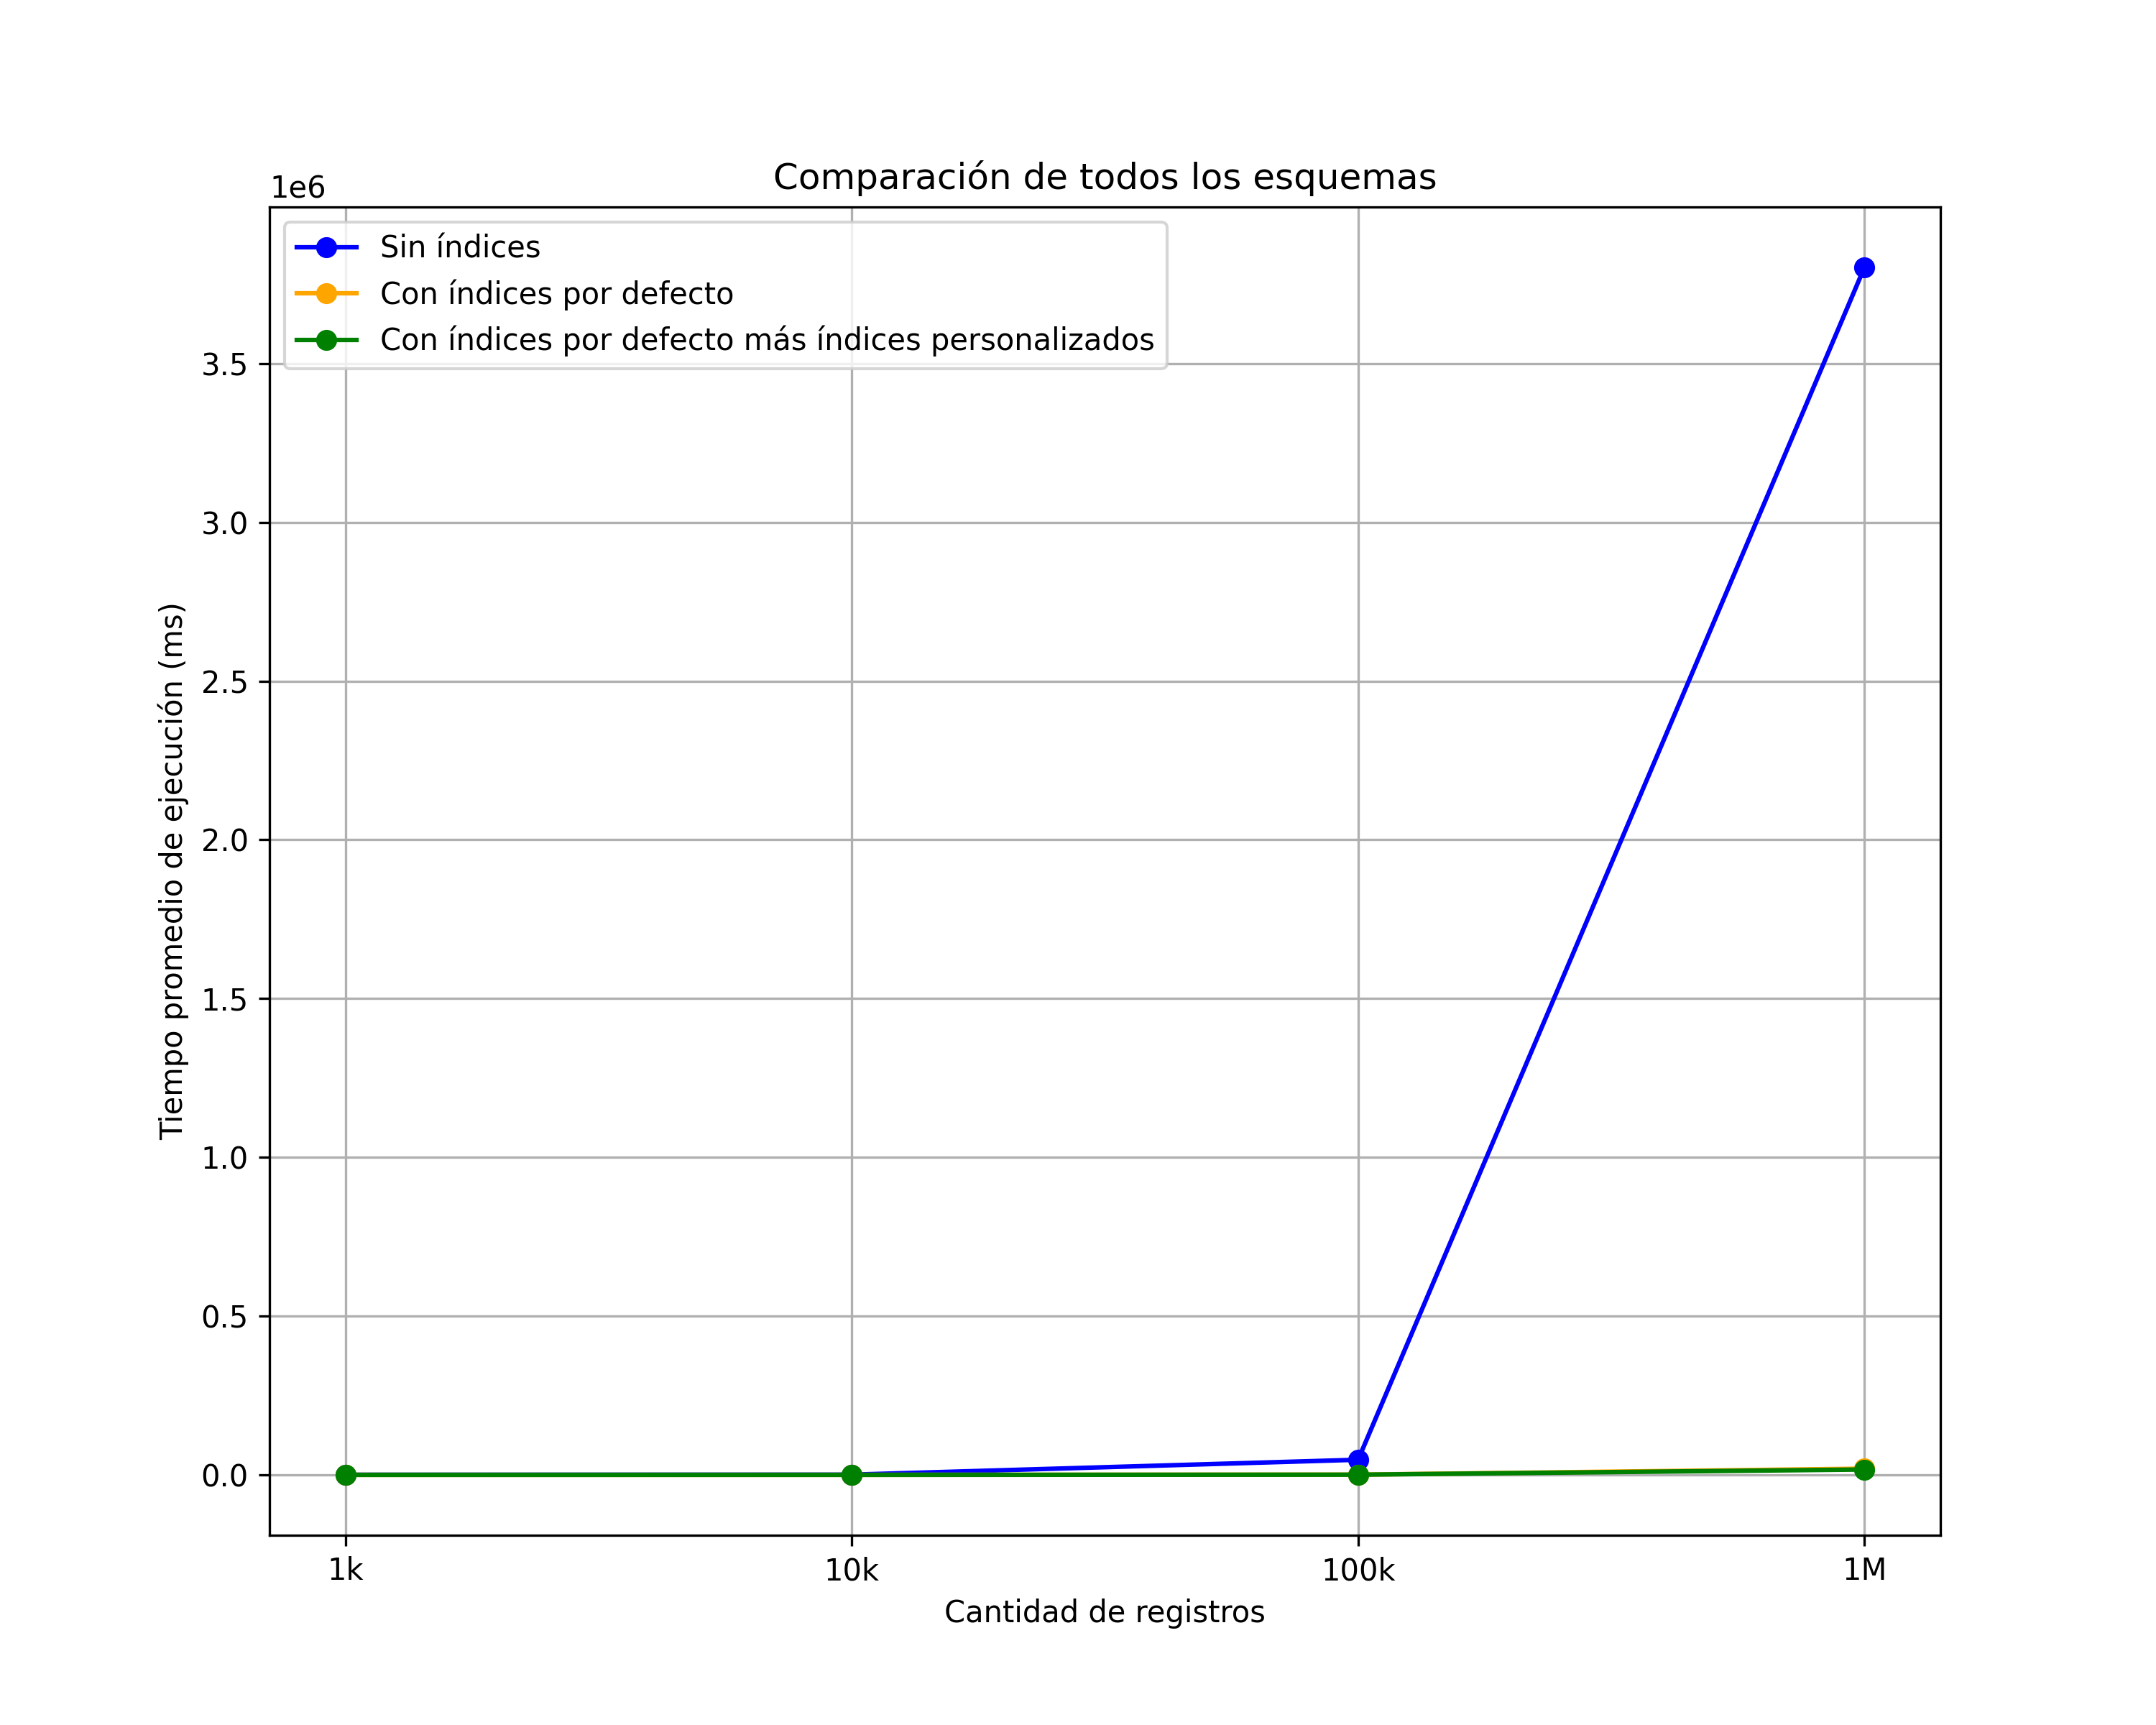
\includegraphics[width=\linewidth, keepaspectratio]{figures/query_2_execution_times_1.png}
	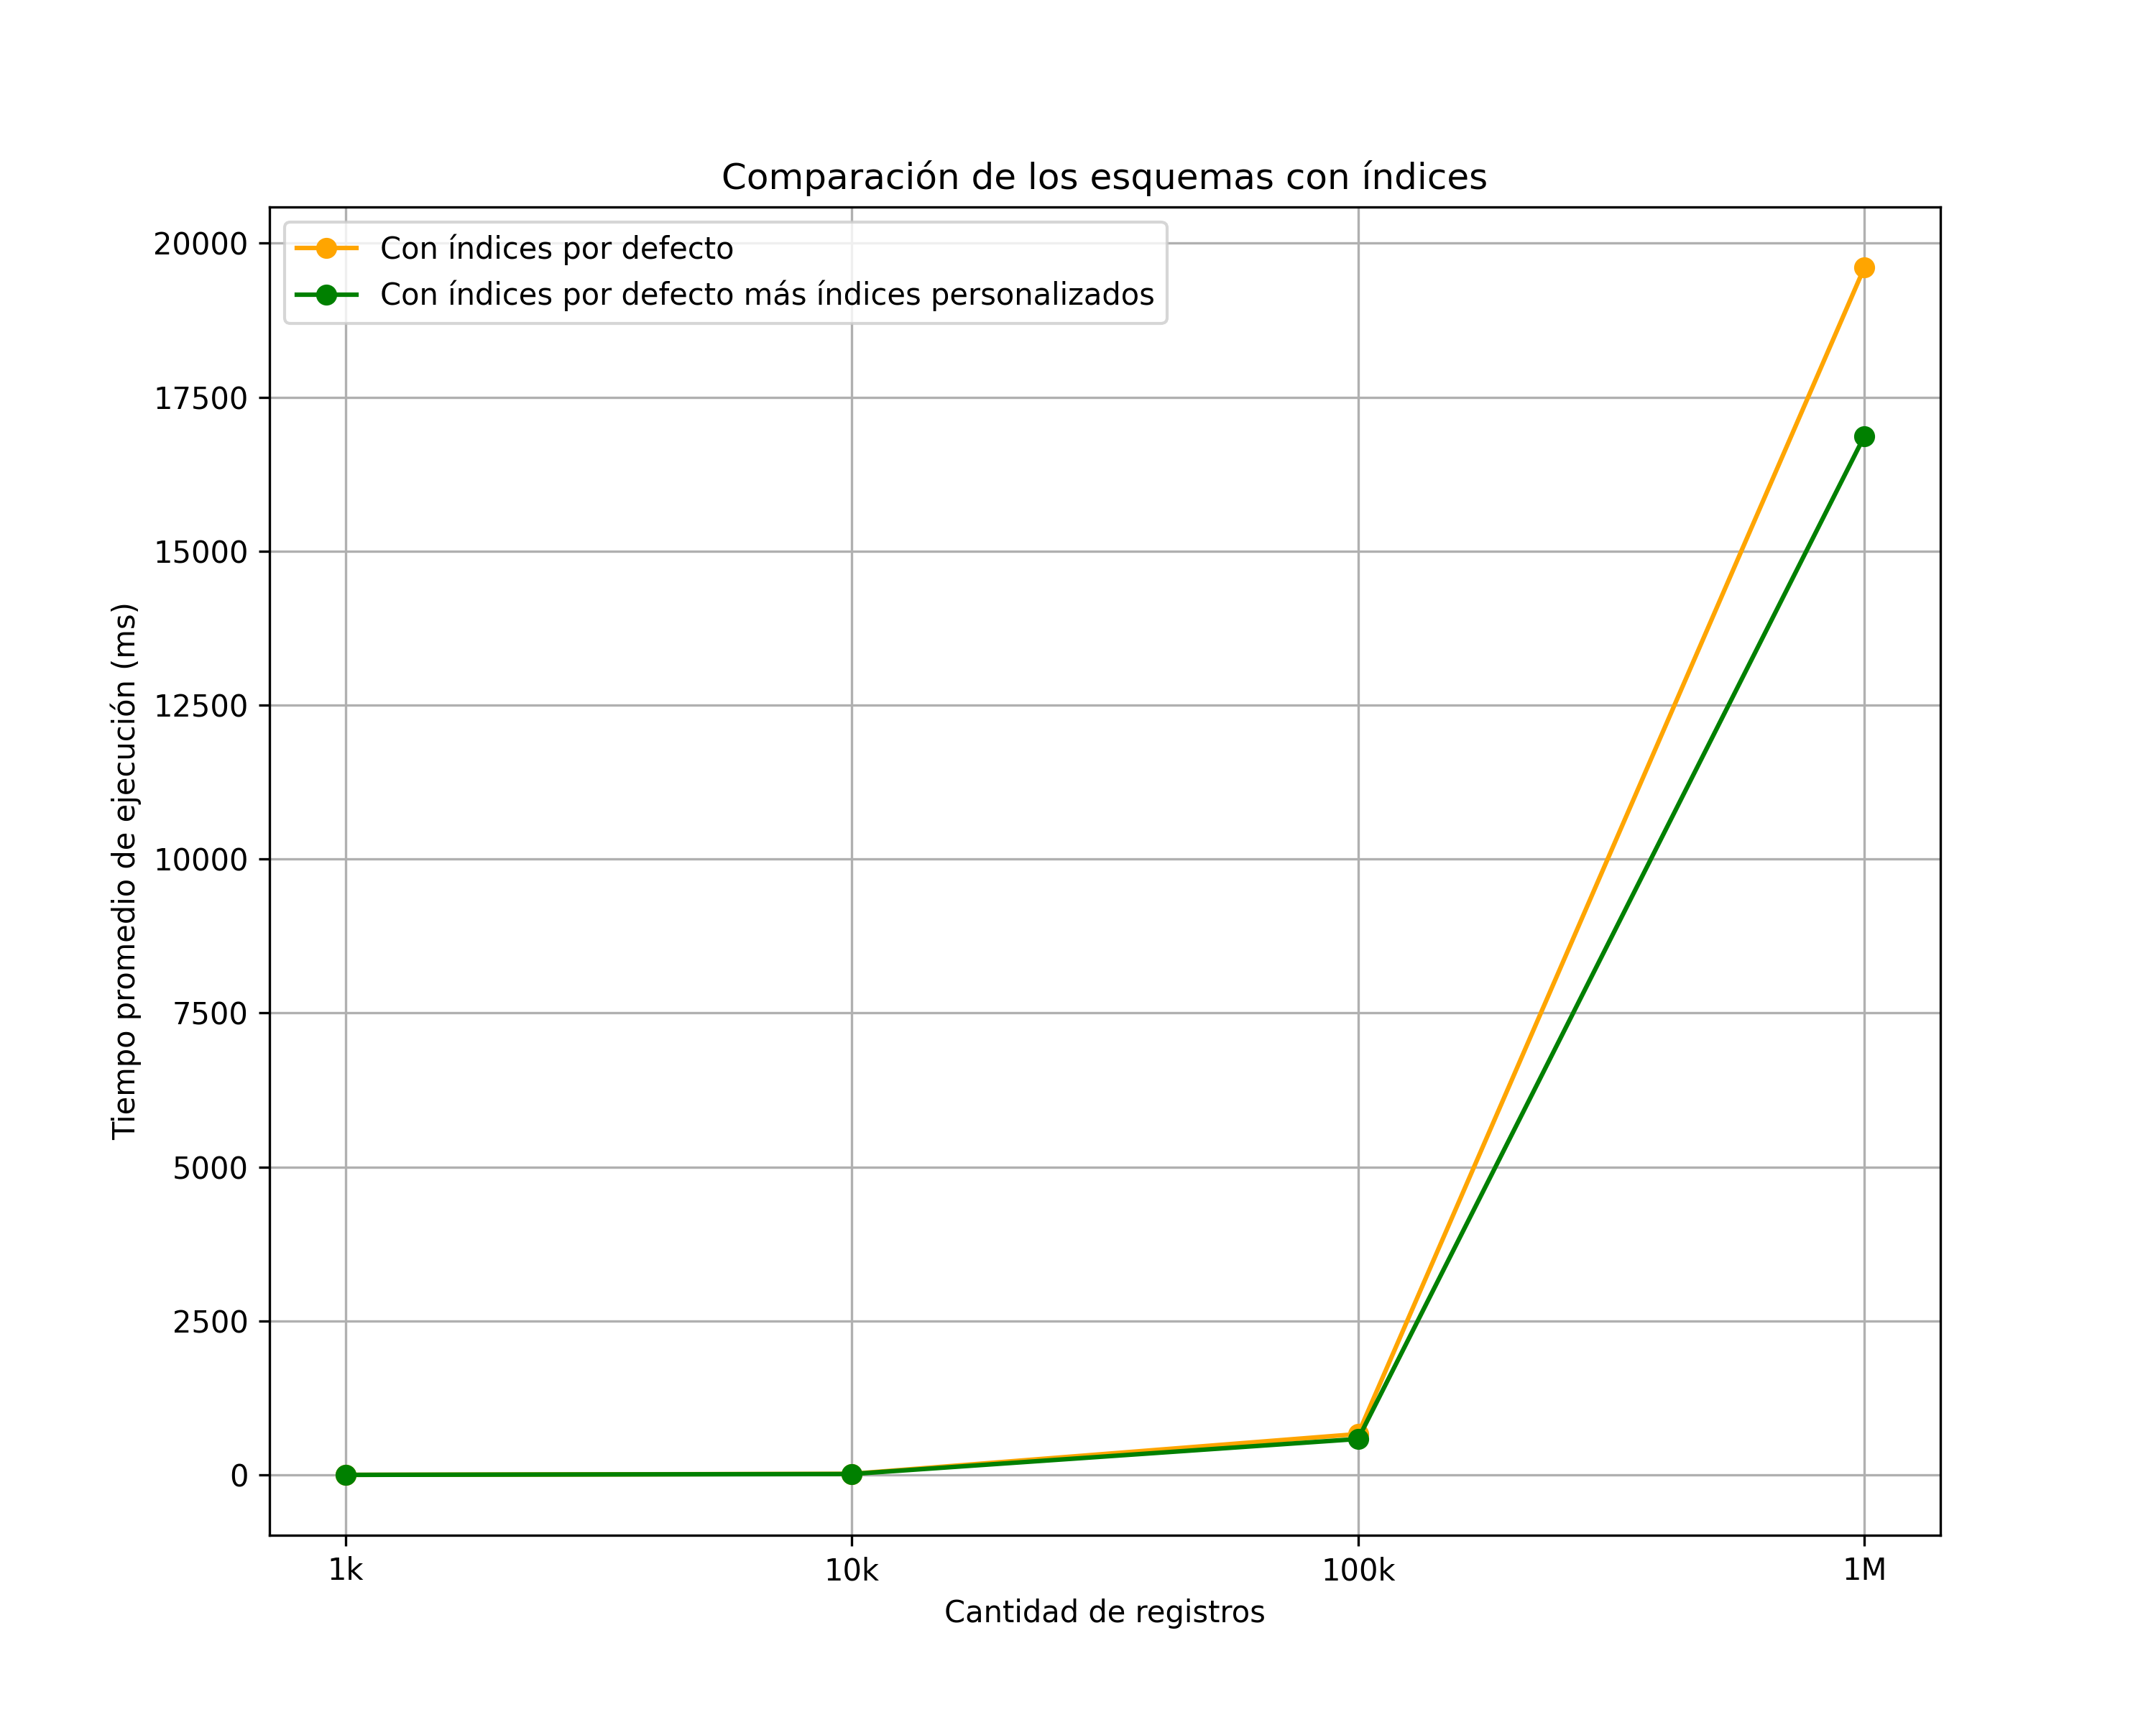
\includegraphics[width=\linewidth, keepaspectratio]{figures/query_2_execution_times_2.png}
\end{center}
En el caso de la segunda consulta, observamos una evidente mejora en los tiempos de ejecución de las consultas con índices: estos optimizan el acceso y filtrado de datos, siendo estas mejoras más pronunciadas en el esquema de un millón de registros. Sin índices, la consulta realiza escaneos secuenciales y uniones anidadas, resultando en tiempos de ejecución muy elevados debido a la cantidad de comparaciones necesarias. Sin embargo, al activar los índices por defecto, se logró una reducción del 99.50\% en el tiempo de ejecución mediante escaneos de índice y uniones hash. Aún así, la mayor eficiencia se obtuvo al implementar un índice en persona.nacimiento\_fecha (más los índices por defecto), disminuyendo el tiempo de ejecución en un 13.91\% comparado con las consultas con índices por defecto. Esta optimización se debe a que el índice específico facilita la búsqueda rápida y reduce significativamente las filas a evaluar. Además, el uso de uniones hash y la reducción de operaciones de materialización contribuyeron a este rendimiento mejorado.
\subsubsection{Consulta 3}
\begin{center}
	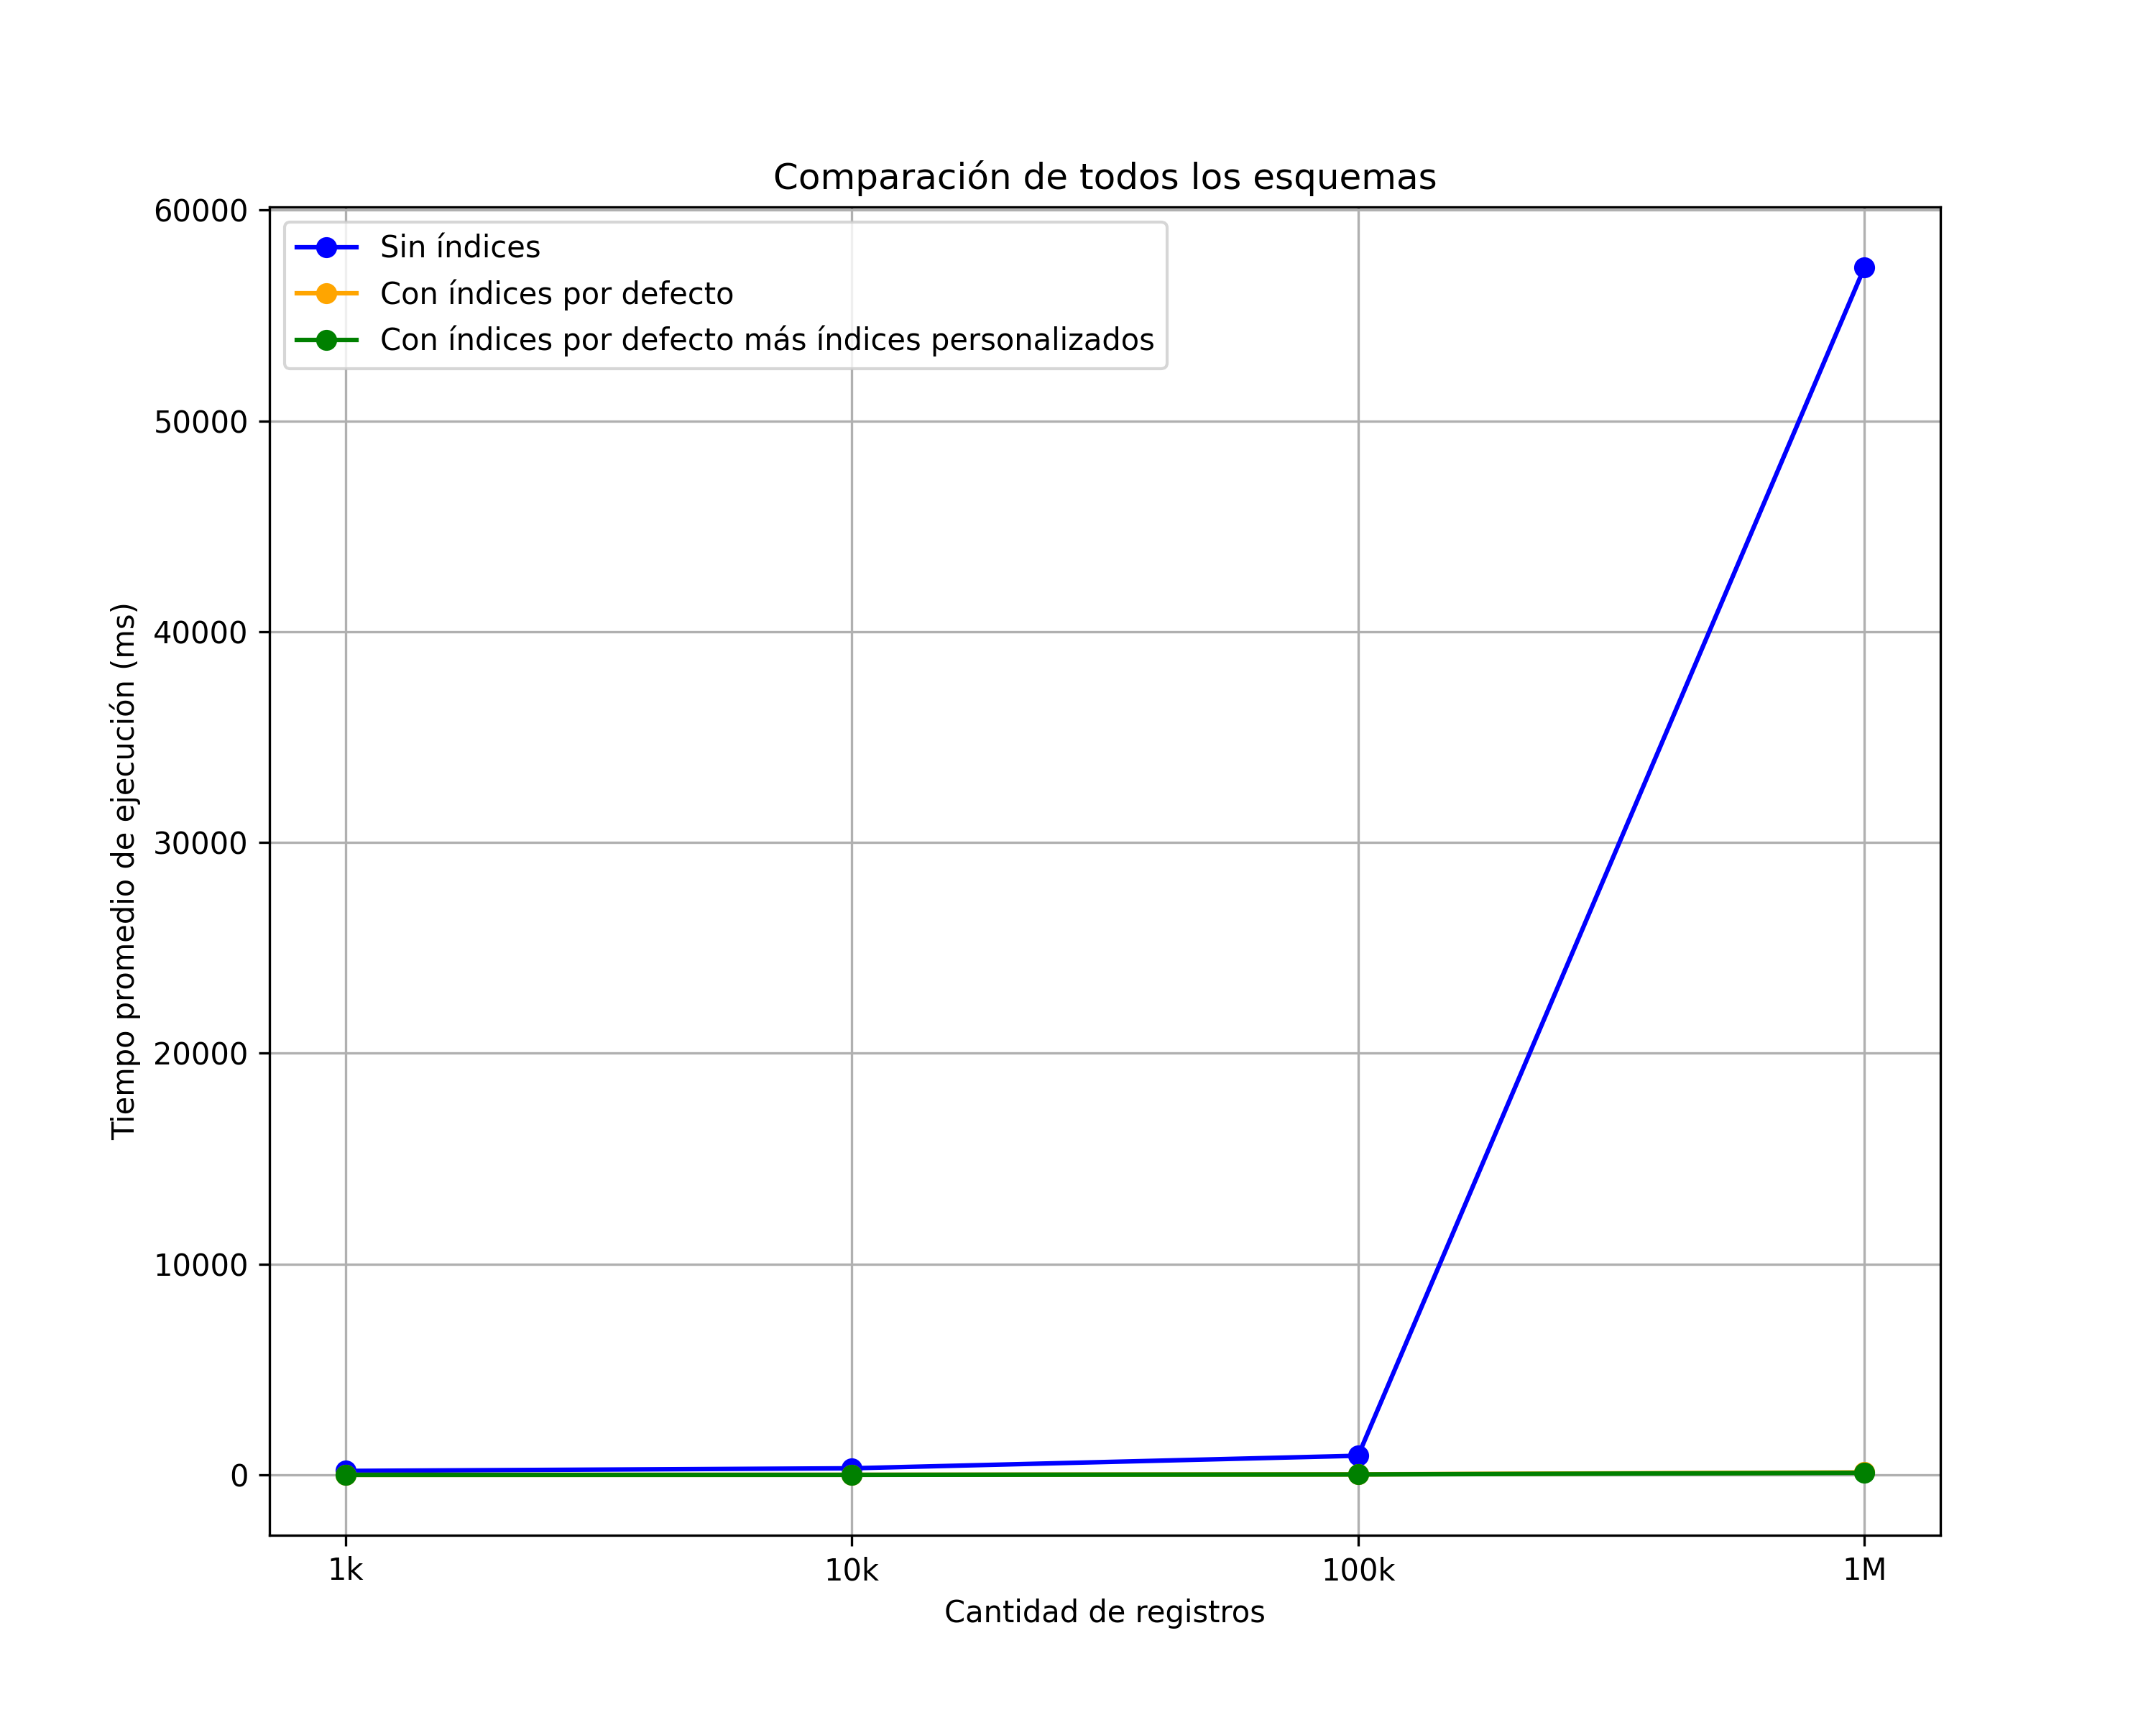
\includegraphics[width=\linewidth, keepaspectratio]{figures/query_3_execution_times_1.png}
	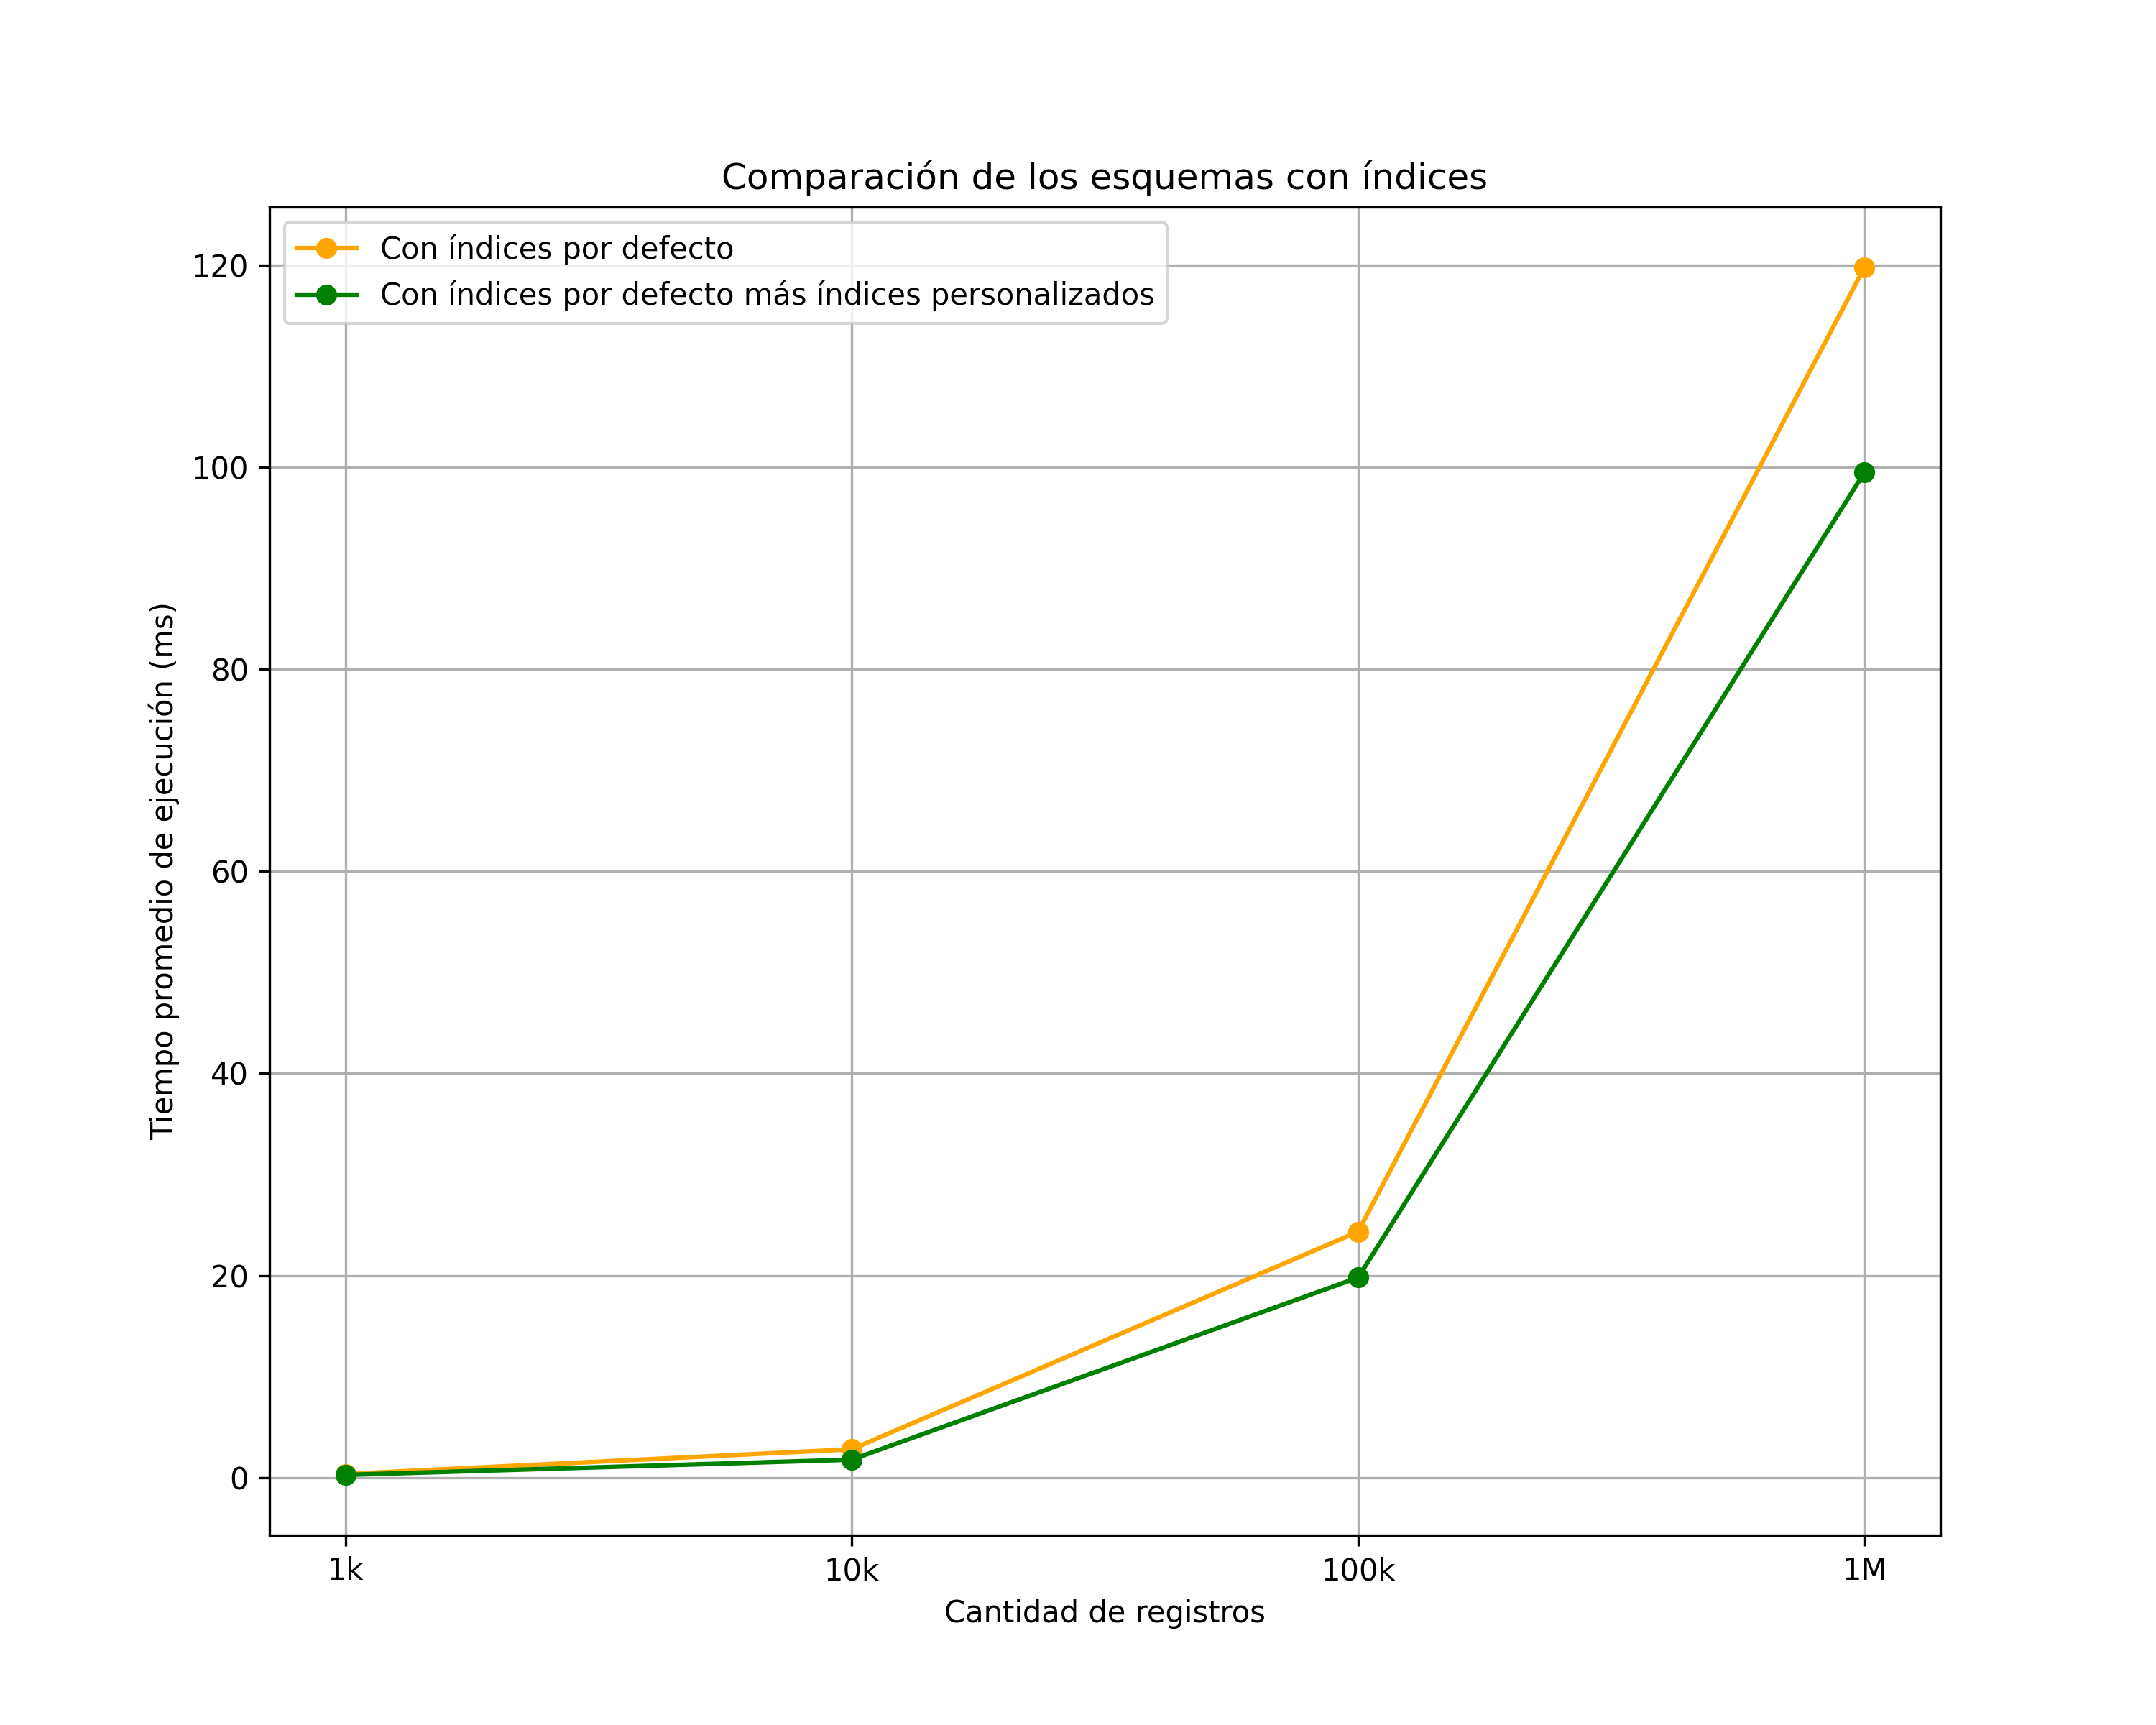
\includegraphics[width=\linewidth, keepaspectratio]{figures/query_3_execution_times_2.png}
\end{center}
Por último, en la tercera consulta —como en las dos anteriores— existen mejoras notables en los tiempos de ejecución de las consultas con índices, especialmente en el escenario de un millón de registros. Sin índices, la consulta depende de escaneos secuenciales y uniones anidadas, lo que resulta en tiempos elevados por la gran cantidad de comparaciones. Al utilizar índices por defecto, logramos una reducción del 99.79\% en el tiempo de ejecución gracias a escaneos de índice y uniones hash. La optimización máxima la alcanzamos al implementar un índice en colaborador.horas\_semanales\_trabajo, reduciendo el tiempo de ejecución en un 16.95\% adicional respecto a los índices por defecto. Esta mejora se debe a que el índice específico agiliza la búsqueda y disminuye considerablemente las filas a evaluar. Además, el empleo de uniones hash en lugar de anidadas y la menor necesidad de materialización de datos contribuyeron a este rendimiento superior. Aunque en volúmenes menores también se observan mejoras, estas no son tan marcadas como en el caso de 1 millón de registros, donde la efectividad del índice es evidente.